% CQL Grid Search: Agreement-Reward Tradeoff
% Replaces: tab:cql-grid-search in section_fourth_down_cql.tex
% Scatter plot showing two distinct optima (conservative vs aggressive)

\begin{figure}[htbp]
\centering
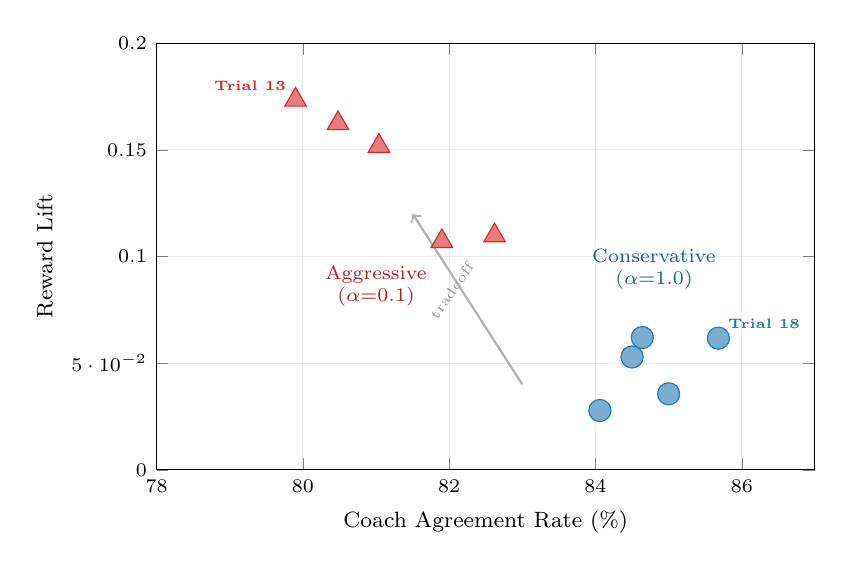
\begin{tikzpicture}
\definecolor{colCons}{RGB}{31,119,180}
\definecolor{colAggr}{RGB}{214,39,40}

\begin{axis}[
  width=0.82\textwidth,
  height=7cm,
  xlabel={Coach Agreement Rate (\%)},
  xlabel style={font=\footnotesize},
  ylabel={Reward Lift},
  ylabel style={font=\footnotesize},
  xmin=78, xmax=87,
  ymin=0, ymax=0.20,
  xticklabel style={font=\scriptsize},
  yticklabel style={font=\scriptsize},
  grid=major,
  grid style={gray!15},
]

% Conservative cluster (alpha=1.0, blue)
\addplot[only marks, mark=*, mark size=4pt, colCons, fill=colCons!60] coordinates {
  (85.68, 0.0617) (85.00, 0.0356) (84.64, 0.0620) (84.50, 0.0529) (84.06, 0.0278)
};

% Aggressive cluster (alpha=0.1, red)
\addplot[only marks, mark=triangle*, mark size=4.5pt, colAggr, fill=colAggr!60] coordinates {
  (79.90, 0.1734) (80.48, 0.1624) (81.04, 0.1517) (82.62, 0.1098) (81.90, 0.1071)
};

% Labels for best in each cluster
\node[font=\tiny\bfseries, text=colCons, anchor=south west] at (axis cs:85.68,0.0617) {Trial 18};
\node[font=\tiny\bfseries, text=colAggr, anchor=south east] at (axis cs:79.90,0.1734) {Trial 13};

% Cluster labels
\node[font=\scriptsize, text=colCons!80!black, anchor=south, align=center] at (axis cs:84.8,0.08)
  {Conservative\\($\alpha{=}1.0$)};
\node[font=\scriptsize, text=colAggr!80!black, anchor=north, align=center] at (axis cs:81.0,0.10)
  {Aggressive\\($\alpha{=}0.1$)};

% Arrow showing tradeoff
\draw[->, thick, black!30] (axis cs:83,0.04) -- (axis cs:81.5,0.12);
\node[font=\tiny, text=black!40, rotate=55, anchor=south] at (axis cs:82.2,0.08) {tradeoff};

\end{axis}
\end{tikzpicture}
\caption[CQL agreement-reward tradeoff]{CQL grid search reveals two distinct optima across 20 configurations. Conservative policies ($\alpha{=}1.0$, blue circles) maximize coaching agreement (85.7\%) but sacrifice reward lift. Aggressive policies ($\alpha{=}0.1$, red triangles) maximize reward (+0.17) but diverge from coaching behavior. Trial 18 ($\alpha{=}1.0$) selected for production: coaches' implicit risk-aversion better reflects real constraints.}
\label{fig:cql-agreement-reward-chart}
\end{figure}
